\section{Methodik, @Tobias Krug}
\subsection{Schemata}
\subsection{Automatisierung}
\subsection{Ausführungsumgebungen für Tests}

\section{Analyse \& Diskussion, @Till Huelder}
\subsection{Vergleich der Schemata}
\subsection{Vergleich der Ausführungsumgebungen}

\section{Thesen, @Tobias Klama}
\subsection{Es besteht eine Korrelation RAM mit world\_size}

Wie zu erwarten steigt der gesamte RAM-Bedarf mit steigender world\_size. Insbesondere bei Schema 1 und 3 liegt jedem Processor
die gesamte Datenmenge vor.
Schema 2 teilt die Daten in Blöcke auf und scattert diese an alle ranks. Diese Aufteilung und dadurch, dass rank\_0 auch an sich selbst
scattert führt dazu, dass rank\_0 einen höheren RAM Bedarf hat als bei Schema 1 und 3. Weiterhin kann den Messungen entnommen werden,
dass ab einer world\_size der gesamt benötigte RAM Bedarf von Schema 2 niedriger als bei den anderen beiden Schemas ist und darüber
hinaus langsamer ansteigt.
Das liegt daran, dass jeder rank nur einen Bruchteil entsprechend der world\_size der Daten erhält und somit jede Vergrößerung der
world\_size einen niedrigeren durchschnittlichen RAM Bedarf ergibt.

\subsection{Es besteht eine Korrelation runtime mit com\_interval}

Das com\_interval ist der Parameter, der angibt wie oft Ranks miteinander kommunizieren.
Anhand der Diagramme TODO einfügen Scatter Plots
ist eine klare Korrelation zwischen der benötigten runtime zur Konvergenz und com\_interval erkennbar.
Eine geringere Häufigkeit der Kommunikation zwischen den Processors führt dazu, dass weniger Zeit für eben diese Kommunikation
verwandt wird und die runtime dadurch sinkt. Im Gegensazt dazu führt ein größeres com\_interval dazu, dass durch das seltenere
Update des J-Vektors die Konvergenz beinträchtigt wird. Das führt zu einer höheren benötigten Iterationsanzahl was schlussendlich
zu einer längeren Laufzeit führt. Der ansteigende Bedarf an Iterationen bei steigendem com\_interval ist in Fig \ref{fig:ScatStepCom}
dargestellt.
Diese beiden sich gegensätzlichen Effekte haben in Summe bei com\_interval 2 und 3 ihr Minimum.

\begin{figure}[h]
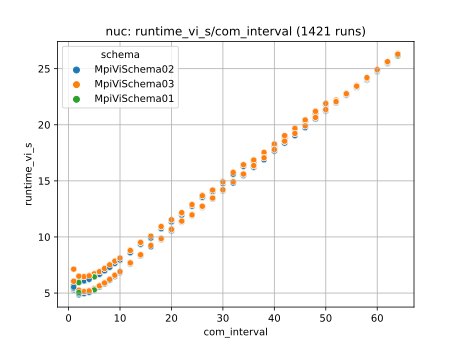
\includegraphics[width=0.5\textwidth]{./gen/img/nuc/small/scatterplot_com_interval_runtime_vi_s.pdf}
\caption{NUC, runtime vs. com\_interval, world\_size 2 \& 4}
\label{fig:ScatRunCom}
\end{figure}

\begin{figure}[h]
\subfloat[HPC class A, runtime vs. world\_size]{
    	\begin{minipage}[c][1.05\width]{
    	   0.23\textwidth}
    	   \centering
    	   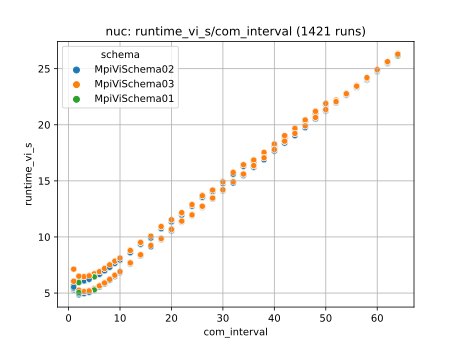
\includegraphics[width=1.1\textwidth]{./gen/img/nuc/small/scatterplot_com_interval_runtime_vi_s.pdf}
    	\end{minipage}}
    	\hfill
\subfloat[HPC class B, runtime vs. world\_size]{
    	\begin{minipage}[c][1.05\width]{
    	   0.23\textwidth}
     	   \centering
     	   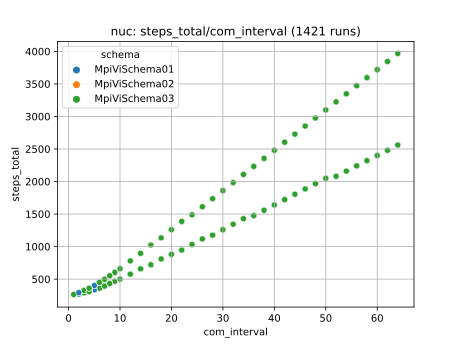
\includegraphics[width=1.1\textwidth]{./gen/img/nuc/small/scatterplot_com_interval_steps_total.pdf}
     	   \label{fig:ScatStepCom}
     	\end{minipage}}
\end{figure}

\subsection{Es besteht eine inverse Korrelation zwischen world\_size und runtime}

Eine größere world\_size sorgt für eine größere Anzahl an Berechnungen, die parallel durchgeführt werden.
Sind die Berechnungen pro Processor komplex/lange genug um den Mehraufwand an inter-Processor Kommunikation zu
gerechtfertigen so führt das zu einer veringerten runtime.
In der vorliegenden Value-Iteration ist der Effekt nicht besonders stark, da die Berechnungen für die nötige
Konvergenz nicht völlig unabhängig voneinander durchgeführt werden können. Das führt zu einer notwendigen Kommunikation,
die dem Effekt der Parallelisierung entgegenwirkt.

Anhand der Messergebnisse kann kein eindeutiger Zusammenhang zwischen der world\_size und der runtime festgestellt werden ref Fig TODO.

Die Auswirkung einer größeren world\_size fällt von Target zu Target unterschiedlich aus.

Bei den isolierten Targets NUC, RPi und Local kann eine geringfügig schnellere Ausführung bei größerer world\_size beobachtet werden.
Das entspricht den zuvor beschriebenen Überlegungen.

Bei den HPC Klassen kann, bis auf world\_size 56 bei HPC Class mixed, beim kleinen Datensatz eine leichte Tendenz zur schnelleren
Ausführung bei größerer world\_size beobachtet werden. Beim normalen Datensatz ist kein Zusammenhang mehr erkennbar.
Das liegt vermutlich daran, dass die HPCs frei zugänglich sind und die Wahrscheinlichkeit weiterer Nutzer, die die runtime
stören, mit steigender world\_size und grundsätzlich längerer Berechnungsdauer durch den größeren Datensatz steigt.
Für eine eindeutige Aussage diesbezüglich sind Messungen mit garantiert freiem Cluster und kontrollierten Störungen nötig.

\section{Beiträge}
- Testumgebung für automatisierte Analyse von Open MPI Kommunikationsschemata für asynchrone Value Iteration auf verschiedenen Ausführungsumgebungen
